
%----------------------------- VARIATIONAL GAUSSIAN PROCESS LATENT VARIABLE MODELS ---------------------------------------------------
 \section{\label{section:vgplvm}Variational Gaussian Process Latent Variable Models}
 \subsection{\label{section:vgplvmBound} Standard Variational Bayesian Inference}

% The variational framework presented in this section not only enables
% the automatic determination of the model complexity, but also results in a training procedure which is robust 
%to overfitting, since the uncertainty in the latent space is treated in a principled Bayesian manner where the
% latent points are marginalised out.

%MAP: a Gaussian process mapping  from a latent space to a data space where the locale of the points in latent 
%space is determined by maximising the Gaussian process likelihood with respect to X.

Given a set of observations $Y$, we assume that these data can be generated by a family of models
$p(Y, \Theta)$, where $\Theta$ is a set of unknown random variables upon which the models depend.
Maximum likelihood approaches seek to find the best model by maximizing the logarithm of the likelihood
$p(Y|\Theta)$ and obtaining a single point estimate for the variables $\Theta$. On the other hand,
Bayesian methods seek to compute the logarithm of the \emph{marginal} likelihood (or evidence) $p(Y)$ according to:
$$
\log p(Y) = \log \int p(Y, \Theta) \intd \Theta  = \log \int p(Y | \Theta) p(\Theta) \intd \Theta.
$$
This approach is advantageous because all possible settings for $\Theta$ are averaged out
while we obtain a posterior distribution $p(\Theta | Y)$ for the unknown variables,
something which leads to an automatic Occam's razor which penalizes complex models
and prevents overfitting.
However, for most interesting models the above integral is intractable, and variational
methods are often employed for approximating this quantity \citep{bishop}. These approaches seek to
lower bound the logarithmn of the model evidence with a functional $\F\left(q(\Theta), Y, \bftheta \right)$
which depends on a variational distribution $q(\Theta)$, the training data $Y$ and the model hyperparameters
$\bftheta$\footnote{Recall that, similarly to the rest of our expressions, $p(Y,\Theta)$ is a
simplified notation for $p(Y,\Theta | \bftheta)$.}. In the rest of the paper the conditioning of the bound 
on the model hyperparameters is dropped for simplicity, like in the rest of our expressions.
The lower bound is obtained
 by applying Jensen's inequality:
\begin{align}
\log p(Y) &= \log \int p(Y, \Theta) \intd \Theta
               = \log \int q(\Theta) \frac{p(Y, \Theta)}{q(\Theta)} \intd \Theta \nonumber \\
               & \geq \int q(\Theta) \log \frac{p(Y, \Theta)}{q(\Theta)} \intd \Theta
                  = \F \left( q(\Theta),Y \right) \label{jensensGeneral} ,
\end{align}
%where we use the notation $q_\Theta = q(\Theta)$.
Mean-field methodologies assume further approximations by letting
the variational distribution factorise with respect to groups of elements
belonging to $\Theta$. 
In any case, $q(\Theta)$ is variationally optimised to approximate the true
posterior $p(\Theta | Y)$ as the bound becomes tighter, \ie as $\F \left(q(\Theta),Y \right)$
approximates $\log p(Y)$. This can be confirmed by observing that
when $q(\Theta) = p(\Theta | Y)$, in equation \eqref{jensensGeneral},
the bound becomes exact.

In the following section we attempt to apply the variational methodology described above
for treating the GP-LVM in a Bayesian manner. We will
explain why this standard approach is inadequate
and will introduce further approximations which lead to an
analytical lower bound.


\subsection{\label{section:vgplvmBound} Variational Inference for the GP-LVM}

A Bayesian treatment of the GP-LVM requires the computation of the log. marginal likelihood
associated with the joint distribution of equation \eqref{joint}.
Since our Bayesian framework will enable automatic dimensionality selection, as will be
explained later in more detail, we opt for an ARD covariance function as was discussed
in section \ref{mapCriticism}.
Both sets of unknown
random variables have to be marginalised out: the mapping values $F$ (as in the standard model)
and the latent space $X$.
Thus, the required integral is written as:
\begin{align}
\log p(Y) &= \log \int p(Y, F, X) \intd X \intd F
                  =  \log \int p( Y | F) p(F | X ) p(X) \intd  X \intd F \label{marginalLikelihood} \\
              &= \log \int p(Y|F) \left( \int p(F|X) p(X) \intd X \right) \intd F \label{marginalLikelihood2}.
\end{align}

%\par The first step in defining a Bayesian treatment for GP-LVM, is to place a prior distribution $p(X|\bftheta_x)$ over the latent space,
%where $\bftheta_x$ denotes any parameters associated with this prior.
%For the moment we will not assume any particular form for this distribution. 
%The set of model parameters now becomes $\bftheta = \{\bftheta_f, \bftheta_x, \beta\}$ and, as before,
%will be omitted from our expressions.
%The joint distribution of the model can be written as
%\begin{equation}
%\label{joint}
%p(Y,F, X) = p(Y|F) p(F|X) p(X)= 
% \prod_{d=1}^D  p(\mathbf{y}_d | \mathbf{f}_d) p(\mathbf{f}_d |
% \mathit{X}) p(X),
%\end{equation}
%\noindent where we assume independence in the data features given the latent variables.


\noindent The key difficulty with this Bayesian approach is propagating the prior
density $p(X)$ through the nonlinear mapping. This
mapping gives the expressive power to the model, but simultaneously
renders the associated log. marginal likelihood \eqref{marginalLikelihood} intractable. 
Indeed, the nested integral in equation \eqref{marginalLikelihood2} can be written
as $\int \prod_{d=1}^D p(\bff_d | X) p(X) \intd F$ and substituting the factorised distribution
with the form given in equation \eqref{priorF} reveals the source of inractability.
More specifically, $X$ is appearing non-linearly in the determinant and the inverse of the
covariance matrix $K_{NN}$, because this matrix is constructed by a non-linear covariance function
with input $X$. 

We now invoke the standard variational Bayesian methodology, described in the previous section,
to approximate the marginal likelihood of equation \eqref{marginalLikelihood} with a variational lower bound.
In more detail, we introduce a factorised variational distribution $q(F,X)=q(F)q(X)$ which depends
on the unknown random variables and we apply Jensen's inequality to obtain the lower bound:
\begin{equation}
\log p(Y) \ge %\F(q, \bftheta) =
       %&=\int a(F,X) \log \frac{p(Y,F,X)}{q(F,X)} \intd F \intd X \label{jensens1}
       \int q(F)q(X) \log \frac{p(Y|F) p(F|X) p(X)}{q(F)q(X)} \intd F \intd X . \label{jensens1}
\end{equation}


%\par We now invoke the variational Bayesian methodology to
%approximate the integral. Following a standard procedure
%\cite{bishop}, we introduce a variational distribution $q(\Theta)$ and
%compute the Jensen's lower bound $\F$ on the logarithm of
%\eqref{marginalLikelihood},
%
%\begin{align}
%\F(q, \boldsymbol \theta) = {}&
%	   % {}& \int q(\mathit{\Theta}) \log
%	   %	\frac{p(Y,F,X)}{q(\Theta)} \intd X \intd F = %\nonumber \\
%	     \int q(\mathit{\Theta}) \log 
%		\frac{ p(Y | F) p(F | X ) p(\mathit{X})}
%			 {q(\mathit{\Theta})}  \intd  X \intd F,
% 	    \nonumber \\
% 	      = {}& \sum_{d=1}^D \int q(\Theta) \log \left( p(\bfy_d | \bff_d) p(\bff_d | X) \right) dX d \bff_d -
% 		    \int q(\Theta) \frac{p(X)}{q(\Theta)} dX
%		 \label{jensens1}
%\end{align}
%
%
 %
%where %$\boldsymbol \theta$ denotes the model parameters $\bftheta = \{\bftheta_f, \bftheta_x, \beta\}$ and 
%$\Theta$ denotes any variational parameters
%associated with the specific form of $q(\Theta)$, which will be defined later on.  However,
%the above form of the lower bound is problematic because $X$ (in the
%GP term $p(F|X)$) appears non-linearly inside the kernel matrix
%$K_{NN}$ making the integration over $X$ difficult.
Here, $q(F)$ approximates the true posterior $p(F|Y,X)$ while $q(X)$ approximates the posterior $p(X|Y)$.
However, the above form of the lower bound is problematic, because it contains the expectation
of $\log p(F|X)$ over the distribution $q(X)$ and, as was explained earlier, $X$ appears nonlinearly
in the GP term and cannot be integrated over.
It is, thus, obvious that standard mean field variational methodologies do not lead to an analytically
tractable algorithm.
\todo[inline]{...}

\subsubsection{Lower bound by introducing auxiliary variables}
\par In contrast, our framework allows us to compute
a closed-form Jensen's lower bound
by applying variational inference after expanding the GP prior so as to include auxiliary inducing
variables. Originally, inducing variables were introduced for computational speed ups in GP regression models
\cite{Csato:sparse02,Seeger:fast03,Csato:thesis02,Snelson:pseudo05,Quinonero:unifying05,Titsias:variational09}.
 In our approach, these extra variables are used as in the variational sparse GP method of
\cite{Titsias:variational09} and result in approximations that do not require inverting covariance
matrices evaluated on $X$ because they are defined in an equivalent but more ``convenient''
probability space.

More specifically, we expand the joint
probability model in (\ref{joint}) by including $M$ extra samples (inducing points) of
the GP latent mapping $\bff$, so that
$\bfu_m \in \mathbb{R}^D$ is such a sample. The inducing points are
evaluated at a set of pseudo-inputs $\tilde{X} \in \mathbb{R}^{M
\times Q}$.
%
 % This general strategy is originally used in approximating GP marginal likelihoods, since it allows reducing
 % the computational and storage complexity from $O(N^3)$ to $O(N M^2)$. Certain methods learn the positions of
 % the inducing points by transforming them into additional kernel hyperparameters and optimizing jointly with
 % respect to all the unknown quantities. However, this technique basically changes the model structure, since
 % the GP prior is practically modified.
 % On the other hand, the approach taken here builds on and significantly extends the recent method of
 % \cite{Titsias:variational09}, where the inducing pionts are transformed 
%
The augmented joint probability density takes the form
\begin{align}
p(Y,F, U,X,\tilde{X})  
=& p(Y|F) p(F|U,X,\tilde{X}) p(U|\tilde{X})p(X) \nonumber \\
=& \prod_{d=1}^D p(\mathbf{y}_d | \mathbf{f}_d) p(\mathbf{f}_d | \mathbf{u}_d, X, \tilde{X}) p(\bfu_d | \tilde{X}) p(X)     \label{augmentedJoint}
\end{align}

%where we used the fact that the joint GP prior over function
%values $F$ and $U$ evaluated at inputs $X$ and $\tilde{X}$ factorizes as
%$p(F, U|X,\tilde{X}) = \prod_{d=1}^D p(\bff_d | \bfu_d,X,\tilde{X}) p(\bfu_d | \tilde{X})$. 
where
\begin{align}
p(\bff_d | \bfu_d,X,\tilde{X}) = \mathcal{N}(\bff_d | \bfa_d, K_{NN} - K_{NM} K_{MM}^{-1} K_{MN})
 \; \; \; \text{with} \;\; \bfa_d = K_{NM}K^{-1}_{MM} \bfu_d \label{priorF2}
\end{align}
is the conditional GP prior (see \eg \citep{rasmussen-williams})
and 
\begin{equation}
\label{pfu}
p(\bfu_d|\tilde{X}) = \mathcal{N}(\bfu_d|\mathbf{0},K_{MM})
\end{equation}
is the marginal GP
prior over the inducing variables. In the above expressions, $K_{MM}$ denotes
the covariance matrix constructed by evaluating the covariance function \eqref{priorF}
on the inducing points, $K_{MN}$ is the cross-covariance between the inducing
and the latent points and $K_{NM} = K_{MN}^\T$.
%The augmented probability model is graphically illustrated in figure \ref{fig:bgplvm}.
Figure \ref{fig:bgplvm} graphically illustrates the augmented probability space of our model,
from now on referred to as \textit{Variational GP-LVM}.

\begin{figure}[ht]
\begin{center}
\subfigure[]{
	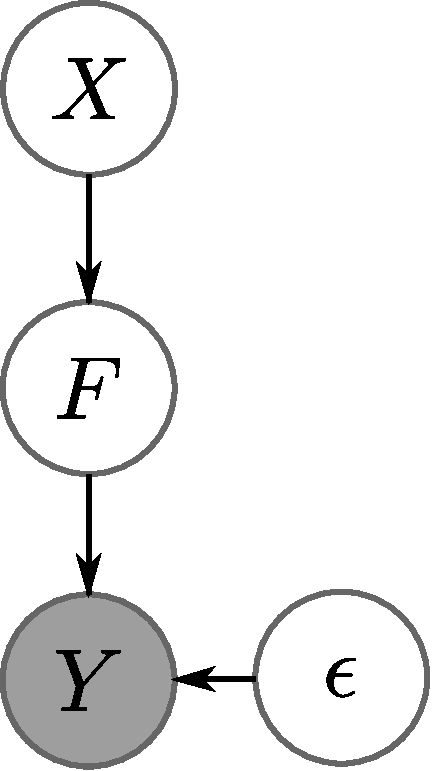
\includegraphics[width=0.12\textwidth]{../diagrams/gplvm}
	\label{fig:gplvm}
}
\hspace{0.1\textwidth}
\subfigure[]{
	\includegraphics[width=0.12\textwidth]{../diagrams/bgplvm}
	\label{fig:bgplvm}
}
%\hspace{0.1\textwidth}
%\subfigure[]{
%	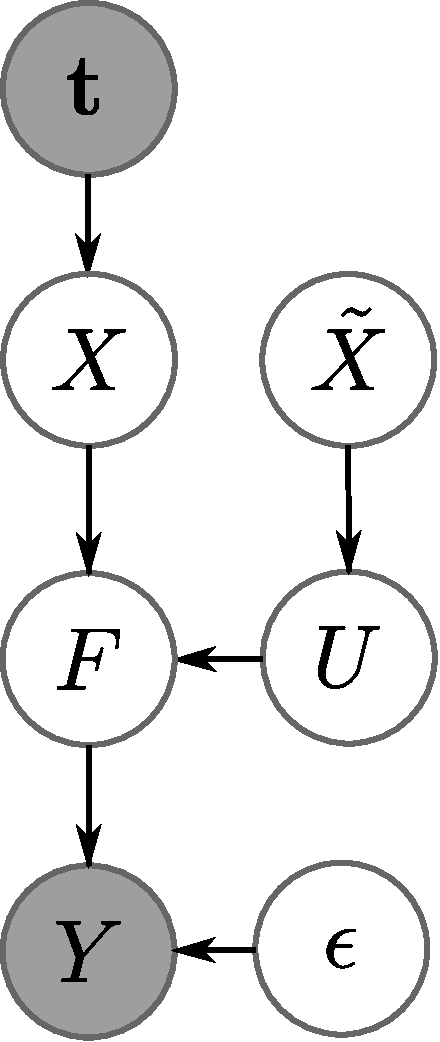
\includegraphics[width=0.12\textwidth]{../diagrams/dbgplvm}
%	\label{fig:dbgplvm}
%}
\end{center}
\vspace{-8pt}
\caption{ \small{
The graphical model for the standard GP-LVM \subref{fig:gplvm} is augmented with auxiliary variables to obtain the
Variational GP-LVM model \subref{fig:bgplvm} %and its dynamical version \subref{fig:dbgplvm}. 
Shaded nodes represent
observed variables.}}
\label{fig:graphicalModels}
\end{figure}



Notice that the likelihood $p(Y|X)$
can be equivalently computed from the above augmented
model by marginalizing out $(F, U)$ and crucially this is
true for any value of the inducing inputs $\tilde{X}$. This means
that, unlike $X$, the inducing inputs $\tilde{X}$ are not random variables.
Neither are they model hyperparameters, they are
variational parameters. This interpretation of the inducing
inputs is key in developing our approximation, it arises
from the variational approach of \cite{Titsias09}. Taking
advantage of this observation we now simplify our notation
by dropping $\tilde{X}$ from our expressions.

We can now
apply variational inference to approximate the true posterior,
$p(F, U | Y, X) = p(F | U, Y, X)$ $p(U | Y, X)$ with
a sparse variational distribution that takes the form
$q(F, U) = p(F | U, X)q(U)$, while the posterior $p(X|Y)$ is still approximated
by the variational distribution $q(X)$ so that, overall:
%
%A key result in \cite{BayesianGPLVM} is that a tractable lower bound (computed analogously to (\ref{jensens1})) can be %obtained through the variational density
%Equation \eqref{jensens1} can now turn into a tractable lower bound through the variational density
\begin{equation}
\label{varDistr}
q(F, U,X) = q(F | U, X) q(U) q(X) = \prod_{d=1}^D p(\bff_d | \bfu_d, X )q(\bfu_d) q(X) .
%q(\mathit{X}, U, F) = p(F | X, U) q(U) q(X)
\end{equation}
%
The distribution $q(X)$ is constrained to be Gaussian:
\begin{equation}
  \label{qX}
  q(X) =  \mathcal{N} \left( X | \mathcal{M}, \mathcal{S} \right)
\end{equation}
%and $q(\bfu_d)$ 
and $q(U)$ is an arbitrary variational distribution.
We can take $q(X)$ to factorise across datapoints or across
features, but this will be further analysed in section
\ref{section:priors} where we discuss the different possible forms of the prior $p(X)$
which, for the moment, is not assumed to have any specific form.

\par The particular choice for the variational distribution
turns equation \eqref{jensens1} into a tractable
lower bound because the nonlinear term of the prior cancels
out with the one of the variational distribution.
Indeed, we can return to
the expression for the lower bound \eqref{jensens1} and
continue our derivation by replacing the joint and the
variational distribution with their augmented versions
(equations \eqref{augmentedJoint} and \eqref{varDistr} respectively) to get:
\begin{align}
\F & \left( q(X), q(U), Y \right) = \int q(F,U,X) \log 
		\frac{ p(Y,F, U,X)}
			 {q(F, U,X)}  \intd  X \intd F \intd U
 	    \nonumber \\
 & = \int \prod_{d=1}^D p(\bff_d | \bfu_d, X )q(\bfu_d) q(X) 
	    \log  \frac{\prod_{d=1}^D p(\mathbf{y}_d | \mathbf{f}_d) \cancel{p(\mathbf{f}_d | \mathbf{u}_d, X)}
						p(\bfu_d)  p(X )}
 	      		   {\prod_{d=1}^D \cancel{p(\bff_d | \bfu_d, X )}q(\bfu_d) q(X)}   \intd  X \intd F  \intd U \nonumber \\
 & = \int \prod_{d=1}^D p(\bff_d | \bfu_d, X )q(\bfu_d) q(X) 
		\log  \frac{\prod_{d=1}^D p(\mathbf{y}_d | \mathbf{f}_d) p(\bfu_d)}
				   {\prod_{d=1}^D q(\bfu_d) q(X)}   \intd  X \intd F  \intd U
-  \int  q(X)   \log \frac{q(X)}{p(X )}   \intd  X \nonumber \\
 & = \hat{\F}\left( q(X), q(U), Y \right) - \KL{q(X)}{p(X)}, \label{jensensSplit}
\end{align}
%
with:
 \begin{align}
\hat{\F} \left( q(X), q(U), Y \right) 
&= 
\sum_{d=1}^D \left( 
    \int q(\bfu_d) q(X) \left\langle \log p(\bfy_d | \bff_d) \right\rangle_{p(\bff_d | \bfu_d, X)} \intd \bfu_d \; \intd X +
					   \log \left\langle \frac{p(\bfu_d)}{q(\bfu_d)} \right\rangle_{q(\bfu_d)} 
  \right) \nonumber \\
  &= \sum_{d=1}^D \hat{\F}_d \left( q(X), q(U), Y \right) . \label{Fd}
\end{align} 

For notational consistency we have dropped the dependency of $\F$ and $\hat{\F}$
on $\bftheta$ and $\tilde{X}$.
The expression in \eqref{jensensSplit} shows that the lower bound can be decomposed in a term which contains
the data ($\hat{\F} \left( q(X), q(U), Y \right)$) and in a term which contains the prior on the latent space
(the $\text{KL}$ quantity). The variational distribution couples these two terms together. In addition,
both of these terms are analytically tractable. The $\text{KL}$ term
%depends on the prior and its calculation
easily calculated for certain priors $p(X)$, and will be discussed in section \ref{}.

%In the next section, we present a detailed derivation of the $\hat{\F}$ term.
%\subsubsection{Detailed derivation of the $\hat{\F}$ term of the bound}

To analytically obtain an expressin for the $\hat{\F} \left( q(X), q(U), Y \right)$ term of the variational bound, we first
marginalise out the auxiliary function values $\bfu_d$ by calculating the
expectation over $p(\bff_d | \bfu_d,X)$ and revealing that the optimal setting for $q(\bfu_d)$ is 
also a Gaussian. More specifically, we have:
\begin{align}
\hat{\F}_d \left( q(X), q(U), Y \right)={}& \int q(\bfu_d) \log \frac{e^{\la \log N \left( \bfy_d | \bfa_d, \beta^{-1} I_d \right) \ra_{q(X)}}
		p(\bfu_d)}{q(\bfu_d)} \intd \bfu_d - \mathcal{A} , \label{boundFAnalytically5}
\end{align}
where $\bfa_d$ is given in equation \eqref{priorF2} and 
$\mathcal{A}=\frac{\beta}{2} \text{tr}(\la K_{NN} \ra_{q(X)}) +
	 	\frac{\beta}{2} \text{tr} \left(K_{MM}^{-1} \la K_{MN} K_{NM} \ra_{q(X)} \right) $.
The expression in \eqref{boundFAnalytically5} is a KL-like quantity and, therefore, $q(\bfu_d)$ is optimally set to be the quantity 
appearing in the numerator of the above equation. So:

\begin{equation}
\label{qu}
q(\bfu_d) = e^{\la \log \mathcal{N} \left( \bfy_d | \bfa_d, \beta^{-1} I_d \right) \ra_{q(X)}}
		p(\bfu_d) ,
\end{equation}
This is a Gaussian distribution since 
$p(\bfu_d )$ is also Gaussian (see equation \eqref{pfu}).

\par We can now re-insert the optimal value for $q(\bfu_d)$ back to the bound's equation and reverse Jensen's inequality to obtain:

\begin{equation}
\label{boundFAnalyticallyFinalIntegral}
\hat{\F_d} \left( q(X), Y \right) = 
	\log \int e^{\la \log N \left( \bfy_d | \bfa_d, \beta^{-1} I_d \right) \ra_{q(X)}}
		p(\bfu_d) \intd \bfu_d -\mathcal{A} .
\end{equation}

\noindent Notice that by optimally eliminating $q(U)$ we obtain a tighter bound which no longer depends on
this distribution, \ie $\hat{\F}_d \left( q(X), Y \right) \geq \hat{\F}_d \left( q(X), q(U), Y \right)$.
Also notice that the expectation appearing in equation \eqref{boundFAnalyticallyFinalIntegral}
is a standard Gaussian integral and \eqref{boundFAnalyticallyFinalIntegral} can
be calculated in closed form, which turns out to be (see supplementary material for details):
\begin{equation}
\label{FdFinal}
\hat{\F}_d \left( q(X), Y \right) = \log \left[   
	\frac{(\beta)^{\frac{N}{2}} \vert \mathit{K_{MM}} \vert ^\frac{1}{2} }
		 {(2\pi)^{\frac{N}{2}} \vert \beta \Psi_2 + \mathit{K_{MM}}  \vert ^\frac{1}{2} } 
	 e^{-\frac{1}{2} \mathbf{y}^{T}_{d} W \mathbf{y}_d}
	 \right]	 -
	 \frac{\beta \psi_0}{2} + \frac{\beta}{2} 
	 \text{tr} \left( \mathit{K_{MM}^{-1}} \Psi_2 \right)	
\end{equation}

\noindent where:
\begin{equation}
\label{psis}
\Psi_0 = \text{tr}(\langle \mathit{K_{NN}} \rangle_{q(\mathit{X})}) \;, \;\;
\Psi_1 = \langle \mathit{K_{NM}} \rangle_{q(\mathit{X})} \;, \;\;
\Psi_2 = \langle \mathit{K_{MN}} \mathit{K_{NM}} \rangle_{q(\mathit{X})}
\end{equation}

\noindent and $W = \beta I_N - \beta^2 \Psi_1 (\beta \Psi_2 + K_{MM})^{-1} \Psi_1^T$. This expression is straight forward to compute, as long as the covariance function $k_f$
 is selected so that the $\Psi$ quantities of \eqref{psis} can be computed analytically. 

It is worth noticing that the $\Psi$ statistics are computed in a decomposable way 
since the covariance matrices appearing in them are evaluated in pairs of
\todo[noline]{This should be written in a better  way}
inputs $\bfx_n$ and $\tilde{\bfx}_m$ taken from $X$ and $\tilde{X}$ respectively.
 In particular, the statistics 
$\psi_0$ and $\Psi_2$ are written as sums of independent terms
where each term is associated with a data point and similarly 
each column of the matrix $\Psi_1$ is associated with only one data point.
This decomposition is useful when a new data vector % is observed
is inserted into the model and can also help to speed up computations during
test time as discussed in section \ref{section:predictions}. 

\todo[noline]{This should be written in a better  way}
%inputs taken from $X$ and $\tilde{X}$, 
Therefore, the averages of the covariance matrices
over $q(X)$ in equation \eqref{psis} of the $\Psi$ statistics
can be computed separately for each marginal
$q(\bfx_n) = \mathcal{N}(\bfx_n | \bfmu_n, S_n)$ taken from the full $q(X)$ of equation \eqref{qX}.
Here, $S_n$ is a vector $\{ S_{n,q}\}_{q=1}^Q$ and constitutes a diagonal
covariance matrix. This matrix is diagonal since the GP-LVM likelihood is
fully factorised, given $f$, something which is obvious from \eqref{generative}.
We can, thus, write that $\psi_0 = \sum_{n=1}^N \psi_0^n$
where
\begin{equation}
\psi_0^n = \int k(\bfx_n,\bfx_n) \mathcal{N}(\bfx_n |\bfmu_n , S_n) d \bfx_n.
\label{eq:psi0}
\end{equation}
Further,
$\Psi_1$ is an $N \times M$ matrix such that  
\begin{equation}
  (\Psi_1)_{nm} = \int k(\bfx_n,\tilde{\bfx}_m) \mathcal{N}(\bfx_n|\bfmu_n, S_n) d
  \bfx_n.
\label{eq:psi1}
\end{equation}
$\Psi_2$ is an $M \times M$ matrix which is written as
 $\Psi_2 = \sum_{n=1}^N \Psi_2^n$ where $\Psi_2^n$ is such that 
\begin{equation}
  (\Psi^n_2)_{m m'} = \int k(\bfx_n,\tilde{\bfx}_m)
  k(\tilde{\bfx}_{m'},\bfx_n) \mathcal{N}(\bfx_n|\bfmu_n, S_n) d \bfx_n.
\label{eq:psi2}
\end{equation}

Notice that these
statistics constitute convolutions of the covariance function $k_f$ with Gaussian densities and 
are tractable for many standard covariance functions, such as the ARD squared exponential or the linear one.
The analytic forms of the $\Psi$ statistics for the aforementioned covariance functions are
given in the appendix.

%Indeed, we can write
%$\psi_0 = \sum_{n=1}^N \psi_)^n$, with
%\begin{align}
%\psi_0^n = \int k(\bfx)
%\end{align}
\todo[inline]{Notice that when $k_f$ is
chosen to be linear, the resulting model can be viewed as an alternative approach to Bayesian PCA \cite{BayesianPCA}). <-
This should go elsewhere}

%Analytic expressions of the $\Psi$ quantities are available in the supplementary material.
%\todo{??? Maybe include $\Psi$ calculations in the main paper??}
%-------------------------

To summarize, the final form of the variational lower bound on the marginal
likelihood $p(Y)$ is written as
\begin{equation}
\F \left( q(X), Y \right) = \hat{\F} \left( q(X), Y \right) - \KL{q(X)}{p(X)}, \label{jensensSplit2}
\end{equation}
where $\hat{\F} \left( q(X), Y \right)$  can be obtained by summing both sides of \eqref{FdFinal} over the
$D$ outputs and the KL term is tractable for specific modelling choices (and is discussed in chapter \ref{}).

 


\subsection{\label{sec:boundSummary}Summary of the variational method and investigation of the lower bound}

Now that the mathematical details of our variational method are explained,
we wish to summarise the method in a higher level and explain how it
compares to the standard variational approaches and to MAP optimisation for the GP-LVM.
Therefore, we start by the objective function of equation
\eqref{gplvmLikelihood} which is traditionally used to train the GP-LVM.
This equation only involves the data $Y$ and the
latent points $X$, since the latent function values $F$ have been
marginalised out. Our framework aims at also marginalising out
the latent points by computing the evidence
$p(Y) = \int p(Y|X) p(X) \intd X$. 
Since we are working on the space where $F$ is marginalised out, we only
consider a variational distribution depending on $X$ and apply Jensen's
inequality to obtain:
\begin{align}
p(Y) \geq \int q(X) \log \frac{p(Y|X)p(X)}{q(X)} \intd X 
	= & \int q(X) \log p(Y|X) \intd X - \KL{q(X)}{p(X)} .
%	 \nonumber \\
	% = & \hat{\F}(q_X, Y) - KL \left[ q(X) \parallel p(X) \right]
\end{align}

In the above quantity, $X$ appears non-linearly in the first term and cannot
be integrated out and, thus, the standard variational approach fails.
By comparing the above equation with the expression of our bound in equation
\eqref{jensensSplit2}, reveals that our framework is, in essence, computing
the following approximation analytically:
\begin{equation}
\label{approxF1}
\hat{\F} \left (q(X), Y \right) \approx \int q(X) \log p(Y|X) \intd X .
\end{equation}
As a by-product, we also obtain an approximate posterior over the latent points
(rather than single point estimates):
\begin{equation}
\label{approxF2}
q(X) \approx p(X|Y) .
\end{equation}

The key to obtaining these approximations is to introduce
auxiliary variables into the model similar to those
used in sparse GP regression.
Therefore, as can be seen from equation \eqref{FdFinal},
the term $\hat{\F} \left( q(X), Y \right)$ is now depending on these extra variables
$\tilde{X}$ appearing inside the covariance matrices $K_{MM}, K_{NM}$.
In particular, we are only required to compute matrix inverses and
determinants which involve $K_{MM}$ instead of $K_{NN}$, something which
is tractable since $K_{MM}$ does not depend on the marginalised quantity $X$.

\todo[inline]{Mention anything about the elimination of q(U)?}

%As already mentioned, the $\Psi$
%quantities appearing in the $\hat{\F}$ term and the KL term of the bound are both
%tractable for specific modelling choices, and their exact expressions are
%derived in sections \ref{PsiQuantities} and \ref{section:priors} respectively.

Investigating more carefully the resulting expression of the bound, 
allows us to gain some intuition regarding
its properties. More precisely, the likelihood term $\hat{\F}_d \left( q(X), Y \right)$,
given in equation \eqref{FdFinal}, 
closely resembles the corresponding sparse GP-LVM
marginal likelihood (where $X$ is optimised rather than being marginalised
out) obtained by applying the variational method of \cite{Titsias:variational09}.
The difference with our results is that in our framework,
$X$ is marginalised out so that the terms containing $X$, i.e. the kernel
quantities $\text{tr}(K_{NN})$, $K_{NM}$ and $K_{NM} K_{MN}$, are transformed
into averages (i.e. the $\Psi$ quantities in \eqref{psi}) with respect to a
variational distribution $q(X)$. Moreover, an extra regularisation term appears
(in the form of the non-negative $\text{KL}$ quantity), which adds constraints
depending on the prior information assumed for $X$.






%The difference is that in our framework an extra regularisation term appears (in the form of the $\text{KL}$ quantity) and also
%the terms that contain $X$, i.e. the kernel quantities $\text{tr}(K_{NN})$, $K_{NM}$ and $K_{NM} K_{MN}$, are transformed into 
%expectations w.r.t a variational distribution, i.e. the $\Psi$ quantities in \eqref{psis}.
%These changes are very natural, since in our work $X$ is marginalised out.

%Although most of the GPLVM-based approaches in the literature assume that $w_i=w_j, \foreach i,j \in \{1,...,Q\}$,
%in this paper we allow a different scale $w_q$ for each latent dimension. This, in combination with the Bayesian
%framework that will be demonstrated later in this paper, enables an automatic relevance
%determination procedure (ARD), i.e.\ it allows Bayesian training to ``switch off'' unnecessary dimensions by
%driving the values of the corresponding scales to zero. In that way, our models are able to find automatically an
%effective number of dimensions for the latent space.

%To summarize, from equations \eqref{varDistr},\eqref{qX} and \eqref{qu} it is obvious that $\{ \mathcal{M}, \mathcal{S}, %\tilde{X} \}$ constitutes the set of variational parameters.
%\footnote{For clarity, from now on we will use the term ``variational parameters'' to only refer to the parameters $\{\mathcal{M}, S\}$ of $q(X)$.}.





%----------------------------------------------- PRIORS ON THE LATENT SPACE ---------------------------------------------------
\subsection{\label{section:priors} Applying the variational framework to different GP-LVM variants}
% -> Allows to capture assumptions
In the previous section we presented a framework for
analytically calculating a variational lower bound on
the logarithm of the marginal likelihood by also
integrating the latent space $X$. For this, we did
not assume any particular form for the prior $p(X)$.
However, the various choices for the form of this density greatly
reflect our overall modelling assumptions and give rise to
models with very different properties, as was discussed in section \ref{section:gplvmDynamics}.

One important advantage of the Variational GP-LVM is that
the variational lower bound includes the prior $p(X)$ in a
simple, separate term which is tractable for many choices of
the prior, as can be seen in equation \eqref{jensensSplit}.
This property allows our framework to be very easily extended
so as to incorporate the specific form of the chosen
latent space prior. 
%In particular, the more complicated 
%$\hat{\F}$ term of equation \eqref{jensensSplit}
%remains the same in all cases and the KL terms is the one that
%has to be computed as appropriate. Further, the variational
%distribution $q(X)$ has to be consistent with the chosen form
%of the prior distribution.
%
In particular, incorporating a specific prior with the
variational framework described in section \ref{section:vgplvmBound}
only requires two additional, simple steps:
firstly, we have to specify a consistent factorisation for $q(X)$
and, secondly, we have to compute the KL term appearing
in the variational bound \eqref{jensensSplit}.
Notice that the more complicated $\hat{\F} \left( q(X), Y \right)$ term is the same
in all cases, exactly as computed in equation \eqref{FdFinal}.

Having these observations in mind, we proceed by demonstrating
the Variational GP-LVM in two very fundamental scenarios.
In the simplest case, the latent space prior is just a standard
normal density factorised across datapoints, as in \eqref{standardNormal}.
In our framework, this scenario can be seen as the non-linear
version of Bayesian PCA \cite{}. 

%as it constrains the latent space $X$ and, indirectly, the data space $Y$ (since the model is generative).
%\par A simple choice is to assign a standard normal density which factorises across datapoints: %, as in \cite{BayesianGPLVM}:
%\begin{equation}
%\label{standardNormal}
%p(X) = \prod_{n=1}^N \mathcal{N}(\bfx_n | \mathbf{0}, I_Q) .
%\end{equation}
%\noindent This prior does not explicitly model correlations between datapoints.
% and, practically, leaves the latent space unconstrainted.
%The fact that our model's likelihood breaks into the two terms shown in \eqref{jensensSplit}, means that incorporating this
%prior with the variational framework described in section \ref{section:vgplvmBound} only requires two additional, easy steps:
%firstly, we have to specify a similar factorisation for $q(X)$, i.e. equation \eqref{qX} can be written in this case as

To incorporate this prior in our framework, we firstly need to let the variational distribution $q(X)$
factorise with respect to datapoints:
\begin{equation}
  \label{qXstatic}
  q(X) = \prod_{n=1}^N \mathcal{N}(\bfx_n | \bfmu_n, S_n).
\end{equation} 
Secondly, the corresponding $\text{KL}$ quantity appearing in \eqref{jensensSplit}  has to be calculated, a task which is
almost trivial, especially given that the covariance matrices $S_n$ (in equation \eqref{qXstatic}) are diagonal. 
More specifically, we find that:
\begin{equation}
\label{KLstatic}
\KL{q(X)}{p(X)} = 
	\frac{1}{2} \sum_{n=1}^N \text{tr} \left( \bfmu_n \bfmu_n^\T + S_n - \log S_n \right)
\end{equation}
The reason why $S_n$ is used to only model variances, is
that the prior for $X$ is a standard normal distribution, i.e a full independence assumption is made for the latent points.
Of course this is not the best modelling approach when it is known a priori that the corresponding observed datapoints $\bfy_n$
are correlated,
%and that's why in the next section we extend our framework for this scenario.
so in the next section we extend the framework for correlated posteriors (see also \cite{Damianou:vgpds11}).

%..important, let's us capture assumptions about y indirectly...



 % \subsection{Using a Static Prior}


%----------------------------------------------- DYNAMIC PRIOR --------------------------------------------------------------------
\subsubsection{\label{temporalPrior} Using a Temporal Prior}

%\todo{Include somewhere a reference to \ref{fig:dgplvm}}
%* Note: include figures from the robot demo, showing the visualisation of the latent space with various kernels.
As already discussed in section \ref{section:gplvmDynamics}, a GPLVM-based dynamical model can be obtained by
additionally including a latent space prior with a temporal component. 
Bayesian inference for such dynamical models is very computationally challenging, as for the standard GP-LVM.
Therefore, practical approaches that have been considered until now
(e.g. \cite{hgplvm, GPDM}) marginalise out only $F$ and seek a MAP solution for $X$.
%
In contrast, our framework allows us to propagate the Gaussian noise through the dynamics
and the latent space of GP-LVM  models with priors of
the form \eqref{priorXgivenT}. 
Therefore, we can approximate the true marginal likelihood $p(Y|\bft)$ of such dynamical models and
obtain an approximate Bayesian solution. 

%The dynamical extension of our
%framework is illustrated graphically in figure \ref{fig:dbgplvm}.
%
%\begin{figure}[ht]
%\begin{center}
%	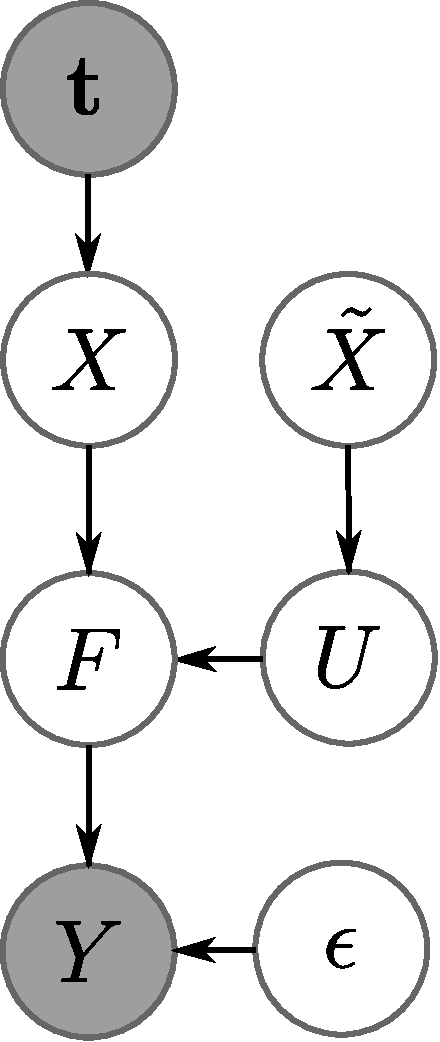
\includegraphics[width=0.12\textwidth]{../diagrams/dbgplvm}
%	\label{fig:dbgplvm}
%\end{center}
%\vspace{-8pt}
%\caption{ \small{
%...}}
%\label{fig:dynBGPLVM}
%\end{figure}


In more detail, we first define a variational distribution $q(X)$ which factorises as:
%
%\par The true marginal likelihood $p(Y|\bft)$ of the above model can be found by extending the framework
%of section \ref{section:vgplvmBound}, since the form of the bound found there, in equation \eqref{jensensSplit}, only contains the
%prior in the $\text{KL}$ quantity as a separate term. Indeed, we can extend our variational framework by first defining a
%variational distribution as in \eqref{varDistr}, but now $q(X)$ factorises as:
\begin{equation}
  q(X) = \prod_{q=1}^Q \mathcal{N} \left( \bfx_q | \bfmu_q, S_q \right)
\end{equation}
%
\noindent in accordance with the temporal prior \eqref{priorXgivenT}. Then,
we find the final form of the lower bound \eqref{jensensSplit} by calculating
the corresponding KL term.
The difference compared to the case when a standard normal prior is used, is that now the covariance matrices 
$S_q$ are no longer diagonal (like the ones appearing in equation \eqref{qXstatic}); instead, the 
posterior over the latent variables now have strong correlations, so $S_q$ is taken to be a $N \times N$ full covariance
matrix. Therefore, 
%although the $\hat{\F}$ term in \eqref{jensensSplit} remains the same for the variational bound of the dynamical GP-LVM model,
the $\text{KL}$ term which contains the prior is now more complicated. More precisely, we find that:
\begin{equation}
\label{KLasSummationOverQ} 
\KL{q(X)}{p(X | \bft)} = \frac{1}{2} \sum_{q=1}^{Q} \left[ 
	  \text{tr} \left( K_t^{-1} S_q 
	                 + K_t^{-1} \boldsymbol \mu_q \boldsymbol \mu_q^T \right)
	  +\log \vert K_t \vert
	  - \log \vert S_q \vert
 \right] - \frac{NQ}{2}.
\end{equation}
As can be seen, a non-factorised distribution $q(X)$ introduces $O(N^2)$ variational parameters,
something which makes optimisation challenging.
%when not factorizing $q(X)$ across data points yields $O(N^2)$ variational parameters to optimize. 
This issue is addressed in the next section.



%\highlight{TODO:} maybe separate section for kernels with images with samples??


%----------------------------------------------- REPARAMETRIZATION AND OPTIMISATION --------------------------------------------
%\subsubsection{Reparametrization and Optimization of the dynamical component \label{optimisation}} 
%Following \cite{OpperFixedPointCovariance}, we can re-express the variational parameters using $K_t$


Recall that a gradient-based algorithm can be employed for training the model, i.e finding the parameters
that maximise the variational lower bound and this optimization procedure
involves the model parameters $\boldsymbol \theta$, the variational
parameters $\{\mathcal{M}, \mathcal{S} \}$ from $q(X)$ and the inducing
points $\tilde{X}$.
%Since $\boldsymbol \theta_f$ and $\boldsymbol \theta_t$ exist in different terms (see \eqref{jensens}), the only coupling between the prior on the latent space (which induces the datapoint correlations) and the likelihood term (which involves observations) is made via the variational parameters. 
% \par In our formulation, unlike \cite{BayesianGPLVM}, the $Q$ variational covariances $S_q$ are full $N \times N$ matrices. 
% Therefore, 
However, when a temporal prior is used, the optimization of the variational parameters 
$\{ \mathcal{M}, \mathcal{S} \} = \{ \bfmu_q, S_q \}_{q=1}^Q$ appears challenging, due to
their large number and the correlations between them. However, by
reparametrizing our $O \left( N^2 \right)$ variational parameters $\{ \mathcal{M}, \mathcal{S} \}$
according to the framework described in
\cite{OpperFixedPointCovariance} we can obtain a set of $O(N)$ less
correlated ones. Specifically, we first take the
derivatives of the variational bound \eqref{jensens1} w.r.t. $S_q$ and
$\bfmu_q$ and set them to zero, to find the stationary
points,
%, one can estimate the variational parameters using fixed-point equations instead of directly optimising them. To obtain such equations we set the variational bound's derivative w.r.t $S_q$ to zero and solve for $S_q$:
\begin{equation}
S_q = \left( \mathit{K}_t^{-1} + \Lambda_q \right)^{-1} \;\;\; \text{and}  \;\;\;  \boldsymbol \mu_q = K_t \bar{\boldsymbol \mu}_q, \label{SFixedPointQ}
\end{equation}
where 
\begin{equation}
\label{lambdaMubar}
\Lambda_q = - 2\frac{\vartheta \hat{\F} \left( q(X), Y)}{\vartheta \mathit{S_q}}
\;\;\; \text{and}  \;\;\;
\bar{\boldsymbol \mu}_q = \frac{\vartheta \hat{\F} \left( q(X), Y \right) }{\vartheta \boldsymbol \mu_q}
\end{equation}
with $\Lambda_q$ being a $N \times N$ diagonal, positive matrix and 
$\bar{\boldsymbol \mu}_q$ being a $N-$dimensional vector.
%It is now obvious that the variational parameters are correlated,
%since they can be re-expressed as a function of $K_t$. 
The above stationary conditions tell us that, since $S_q$ depends on a
diagonal matrix $\Lambda_q$, we can reparametrize it using only the
$N-$dimensional diagonal of that matrix, denoted by $\boldsymbol
\lambda_q$.  Then, we can optimise the $2 (Q \times N)$ parameters 
$(\boldsymbol \lambda_q$, $\bar{\bfmu}_q)$ and obtain the original
parameters using \eqref{SFixedPointQ}. 

There are two optimisation strategies, depending
on the way we choose to treat the newly introduced parameters $\bflambda_q$ and $\bfmu_q$.
Firstly, we can follow \cite{OpperFixedPointCovariance} and construct an EM-style algorithm, after observing the dependencies
between the expressions involving the variational bound and the variational parameters.
Indeed, the variational bound $\F$ in equation \eqref{jensensSplit} depends on the variational parameters
$\bfmu_q$ and $S_q$ of $q(X)$, which through equation \eqref{SFixedPointQ} depend on the newly introduced
quantities $\bar{\bfmu}_q$ and $\bflambda_q$ which, in turn, are associated with $\F$
through equation \eqref{lambdaMubar}. These observations lead to the EM algorithm \ref{EMOptimize}, which alternates
between estimating one of the parameter sets $\{\bftheta, \tilde{X} \}$ and $\{ \mathcal{M}, \mathcal{S} \}$ by keeping the other set fixed.

\todo{Remove this algorithm}
\begin{algorithm}
\caption{EM algorithm for optimising the model and variational parameters}
\label{EMOptimize}
\begin{algorithmic}
\STATE Define $\tilde{\bftheta} \triangleq \{\bftheta, \tilde{X} \}$, where $\bftheta$ are the model parameters and $\tilde{X}$ the inducing inputs
\STATE Initialize $\tilde{\bftheta}^k, \{\bfmu_q^{(k)}, S_q^{(k)}\}_{q=1}^Q$ for $k=0$
\STATE $k=1$
\REPEAT
    \STATE $\forall q$ compute $\bar{\bfmu}_q$ and $\bflambda_q$ from equation \eqref{lambdaMubar} 
       for the current value of the bound $\F^{(k-1)}$.
	\STATE $\forall q$ compute $\bfmu_q^{(k)}$ and $S_q^{(k)}$ from equation \eqref{SFixedPointQ}
	 with $\tilde{\bftheta}^{(k-1)}$ held fixed.
	\STATE Compute
	    $\tilde{\bftheta}^{(k)} = \underset{\tilde{\bftheta}}{\operatorname{max}} \F^{(k-1)}(q, \bftheta)$ 
	    from equation \eqref{jensensSplit} with $\bfmu_q^{(k)}$ and $S^{(k)}$ held fixed.
	\STATE Compute the value of the bound $\F^{(k)}$ for the new set of variational and model parameters.
    \STATE $k = k+1$
\UNTIL{convergence}
\RETURN $\tilde{\bftheta}^k, \{\bfmu_q^{(k)}, S_q^{(k)}\}_{q=1}^Q$
\end{algorithmic}
\end{algorithm}

An alrtenative approach, which is the one we use in our implementation, is to treat the new parameters
$\bflambda_q$ and $\bfmu_q$ as completely free ones so that equation \eqref{lambdaMubar} is never used. In this case, the
variational parameters are optimised directly with a gradient based optimiser, jointly with the model
hyperparameters.

It is now obvious why this reparameterization is appealing not only in terms of computational
complexity, but also in terms of optimisation robustness. Indeed, equation \eqref{SFixedPointQ} 
confirms that the original variational parameters are coupled via $K_t$, which is a full-rank covariance matrix
computed for all time points $t_n$. By reparametrizing according to equation \eqref{SFixedPointQ} and treating
the new parameters as free ones, we manage to break this coupling and apply our optimisation algorithm on a
more stable space.

%One important fact which must be emphasized is that, with the aforementioned methodology, each $\boldsymbol \mu_q$ as well as $S_q$ is now re-parametrised using $K_t$ which means that they now include kernel hyperparameters $\boldsymbol \theta_t$; therefore, the quantity $\frac{\partial \mathbf{F}}{\partial \theta_t}$ should be amended with the partial derivatives as appropriate.



\subsection{Optimisation and Bayesian model selection}

The lower bound \eqref{jensensSplit} can be jointly maximized over the
model $\left( \bftheta_f \right)$ and variational parameters $ \left( \{ \mathcal{M}, \mathcal{S}, \tilde{X} \} \right) $
%parameters $\boldsymbol \theta = (\beta, \boldsymbol \theta_f, \boldsymbol \theta_x)$, the variational
%parameters $\{ \mathcal{M}, S \}$ from $q(X)$ and the inducing points
%\footnote{We will use the term ``variational parameters'' to
%  refer only to the parameters of $q(X)$ although the inducing points
%  are also variational parameters.} 
%  $\tilde{X}$ 
by applying a gradient-based optimization algorithm. This approach is
similar to the MAP optimization of the objective function employed in the standard GP-LVM \cite{GPLVM} with the main
difference being that instead of optimizing the random variables $X$, we now optimize a set of \textit{variational
  parameters} which govern the approximate posterior variances in the latent space. The fact that the inducing points
$\tilde{X}$ are not model hyperparameters, means that their presence does not affect the model complexity.
%
%It is now obvious how automatic selection of the latent space dimensionality can be achieved

It is now obvious how our models
are able to find automatically an effective number of dimensions for the latent space:
when the ARD covariance function \eqref{ard} (or the linear ARD function defined in \eqref{linard}) are used for the mapping
$k_f$, the parameter vector $\bftheta_f$ includes the $Q$ different scales $w_q$,
and the Bayesian training is able to ``switch off'' unnecessary dimensions by driving the values of the corresponding
scales to, or close to zero. 
 Notice that this is only possible in a Bayesian framework such as the one presented here;
employing an ARD covariance function for the standard GP-LVM would not cause the same effect for the
reasons explained in section \ref{mapCriticism}.

%\par Figure \ref{fig:bgplvm} shows the graphical representation of our model, from now on referred to as %\textit{Variational GP-LVM}.
%Forcing $X$ to be time dependent, as shown in \ref{fig:dbgplvm}, results in a dynamical version of the model. This is
% explained in more detail in the next section.

\todo{Move some text from \ref{BayesnaModelSelectionExperiments} to here.}


%----------------------------------------------- NUMERICALLY STABLE FORMULATION -----------------------------------------------
%\subsubsection{Numerically stable formulation}
%--> Supplementary
%%%% TODO

